\subsubsection{Results and Future Work}

The results of the lift calculation is presented in Figure \ref{fig:liftCoeff}. As expected, the lift coefficient is constant across a changing Mach number. While this is not representative of a real system, the effect of lift on the SFRJ is minimal due to flying at a low angle of attack, typically less than seven degrees.

\begin{figure}[H]
    \centering
    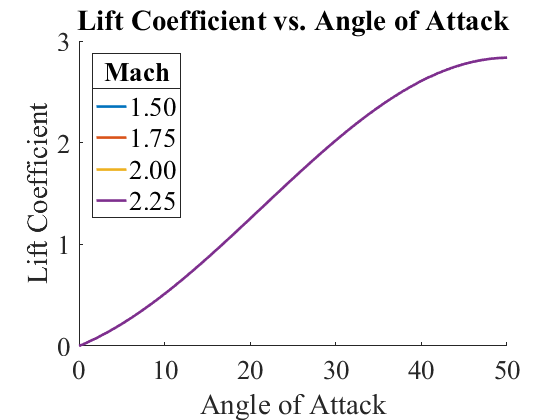
\includegraphics[width=0.7\textwidth]{LiftAndDragAnalysis/figures/LiftCoeffcAoA.png}
    \caption{Lift Coefficient vs. Angle of Attack}
    \label{fig:liftCoeff}
\end{figure}

The results of the drag analysis is shown in the Figure below. At mach 2.5, the SFRJ experiences a drag coefficient of 0.74. In comparison to Twin Intake X-Tail design, which has a drag coefficient of 0.56 at mach 2.5, the SFRJ designed experiences much higher drag values. Drag coefficient also increases as mach increase in the figure which is an unusual trend and thus needs further attention. 

\begin{figure}[H]
    \centering
    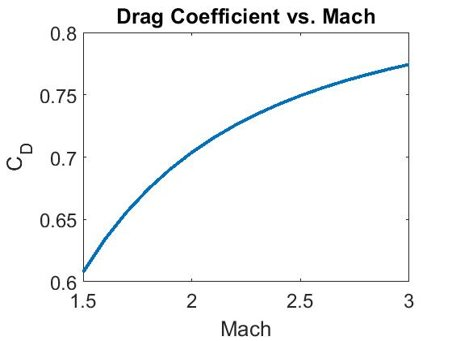
\includegraphics[width=0.7\linewidth]{LiftAndDragAnalysis/DragChart.png}
    \caption{Drag Coefficient vs Mach}
    \label{fig:Drag Coefficient}
\end{figure}

After further analysis of the results, higher drag coefficient and increasing drag  can be attributed to the 2-dimensional equations used to conduct the drag analysis of the Inlet. Since the Inlet has complex 3-dimensional geometry, further analysis using CFD will give a more accurate drag coefficient and thus reduce the overall drag coefficient. In future, further attention to Inlet Spillage Drag and Inlet Cowl Drag using CFD needs to be conducted. 

The drag polar is shown in Figure \ref{fig:dragPolar}. The results are generally as expected, with a peak lift-to-drag ratio near and angle of attack of 25 degrees. Increasing Mach number shows a decrease in the lift-to-drag ratio, which is contradictory to conventional knowledge, but this is a result of the deficiencies of the lift and drag models used. Overall, the peak lift-to-drag ratio approach 1.2, which is near a common approximation of 1.5 \cite{fleeman_2001}. 

\begin{figure}[H]
    \centering
    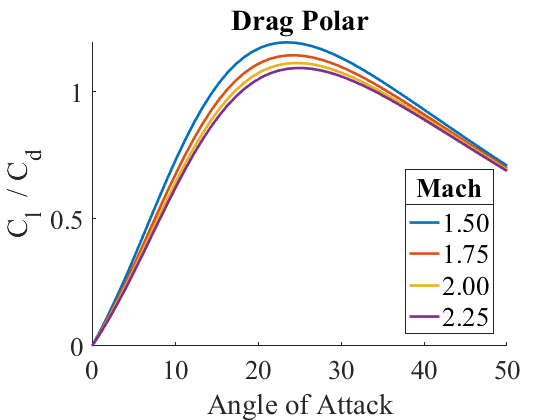
\includegraphics[width=0.7\textwidth]{LiftAndDragAnalysis/figures/DragPolar.png}
    \caption{Drag Polar}
    \label{fig:dragPolar}
\end{figure}

